\chapterimage{chapter_head_1.pdf} % Chapter heading image
\chapter{기상청 일기 예보}

\section{예보가 나오는 과정}

예보가 나오기까지는 기상실황파악 → 자료수집 → 분석 → 예보작성 → 통보 과정을 거친다. 

\section{기상실황 파악}

\subsection{지상기상 관측}
전국 76개소의 기상관서에서 하늘상태, 시정 등의 목측 (目測 ) 요소를 관측하고 있으며, 기온, 습도, 강수량, 바람, 기압 등은 자동기상관측장비를 이용하여 1분 간격으로 관측되고 있다. 또한, 기상관서가 없는 500여 소에서는 방재용 자동기상관측장비를 이용하여 기온, 풍향, 풍속, 강수량, 강수 유무를 1분 간격으로 관측하여 기상실황을 감시하고 있다.

\subsection{항공기상관측}
전국 공항기상관서에서는 바람, 시정, 운고, 기온, 기압 등의 항공기상관측요소를 매30분 또는 1시간 간격으로 관측하며, 활주로에 설치된 공항기상관측장비에 의해 기상요소들이 매분 자동 관측된다. 특히 인천, 제주, 양양, 울산 등의 공항에서는 이·착륙 항공기에 영향을 미치는 저층난류를 탐측하기 위하여 저층난류경보장치를 운영하고 있다.

\subsection{고층기상관측}
고층기상관측은 지상보다 높은 상층 대기의 상태를 관측하는 것으로, 기상청은 레윈존데 관측, 수직측풍장비 관측을 수행한다. 레윈존데 관측은 기구에 라디오존데를 매달아 지상으로부터 약 35 km(5 hPa)까지의 고도별 기압, 기온, 습도, 풍향, 풍속을 00UTC와 12UTC에 관측하며, 수직측풍장비 관측은 UHF나 VHF 파장의 전파를 상층대기로 방사하고 바람과 함께 이동하는 난류에 산란되어 다시 수신되는 전파신호로 바람을 10분 간격으로 관측한다.

\subsection{해양기상관측}
해양기상관서, 해양기상관측부이, 해양기상영상감시시스템을 통하여 풍향·풍속, 기온, 수온, 기압, 파고 등을 관측하며, 먼바다의 기상현상 관측 및 부이 관리를 위하여 기상관측선을 운영하고 있다.

\subsection{기상위성관측}
기상위성은 우주공간에서 지구의 기상변화를 관측한다. 기상청은 정지궤도기상위성과 극궤도기상위성의 자료를 직접 수신하여 처리하여 예보를 위해 사용하고, 국민에게도 공개하고 있다. 이를 위해 기상위성 수신처리분석시스템을 서울, 문산, 서산에 설치하여 운영중이다.

\subsection{기상레이더 관측}
도플러 기상레이더를 설치하여 한반도에서 발생하는 악기상을 관측하여 예보에 활용하고 있다. 또한 일본 기상청과 공군의 레이더 자료도 수신하여 기존영상과 합성하여 종합적으로 활용하고 있다.


\section{자료수집}
통신용컴퓨터를 이용하여 국내기상자료와 외국에서 송신되는 각종기상자료를 수집, 편집, 가공하여 분석용 컴퓨터로 보낸다. 국내·외에서 수집된 관측자료로부터 수치예보모델을 이용하여 예상일기도를 생산한다. 이러한 수치예보모델의 운용을 위해 슈퍼컴퓨터가 사용된다.

<<<<<<< HEAD
\section{일기도 분석}\index{일기도 분석}
=======


\section{일기도 그리기}\index{일기도 그리기}

\subsection{일기도}\index{일기도}
일기도(지상 일기도)는 어느 지역 내의 일기 개황을 한 눈에 보아서 알 수 있도록
각종 기상요소(기압, 습도, 기온, 이슬점, 운량, 풍향, 풍속 등)를 나타낸 것으로 이것을
이용하여 각 지역의 일기를 알 수 있으며, 연속된 일기도를 통해 앞으로의 일기를 예상할 수 있다.

\subsection{관측자료 기입}\index{관측자료 기입}
일기도에 관측된 자료를 나타낼 때에는 <그림 Ⅲ-20>과 같이 정해진 일정한 형식으로 기입해야 한다. 기입이 끝나면 일기도 상에서 기압, 기온 또는 필요한 기상요소들에 대하여 값이 같은 점을 연결하여 선을 긋는다. 일기도에서 가장 중요하게 다루는 선이 등압선이다. 등압선은 기압이 같은 지점을 연결한 선이다. 등압선을 그려보면 고기압과 저기압의 위치, 전선 등을 가려 낼 수 있다. 이것은 마치 지도에 그려진 등고선의 분포모양을 보고 산이나 골짜기를 판별하는 것과 유사하다. 등압선을 그리는 방법은 다음과 같다.
① 주어진 일기도에 기입된 각종 자료 중 구름의 양, 풍향, 풍속, 기압 등의 의미를 파악한다.
기압은 자연 상태에서 보통 1060 hPa을 넘지 않으므로, 첫자리 수가 0에서 5사이이면 10
을, 6에서 9사이이면 9를 각각 앞에 붙여 계산한다.
② 일반적으로 등압선은 1000 hPa을 기준으로 ......, 992, 996, 1000, 1004, 1008, ...... 등 4 hPa 간격으로 그린다. 그러나 등압선 간의 폭이 너무 넓어 기압배치를 파악하기 어려울
때는 2 hPa 간격으로 파선을 그린다.
③ 그리기 쉬운 곳(등압선이 조밀하지 않은 곳)부터 그려 나간다.
④ 등압선은 중간에서 끊어지거나 없어지지 않는다.
⑤ 관측값이 없는 경우는 내삽, 또는 외삽법의 원리로 <그림 Ⅲ-21>과 같이 이웃하는 두 지
점의 간격을 비례로 나누어서 부드럽고 매끈한 곡선으로 그린다.
⑥ 한 선으로 연결되는 등압선은 양쪽 끝에 기압의 값을 기입하고, 폐곡선의 경우는 위쪽(북
쪽) 중앙에 등압선을 끊고 값을 기입한다. 저기압의 중심은 적색으로 L(low pressure), 고
기압의 중심은 청색으로 H(high pressure)라고 표시한다.
일기도가 그려지면 고기압과 저기압의 위치 및 이동경로, 기압과 고도의 변화경향, 전선의
발생 및 소멸과 이동, 날씨변화, 대기의 수직구조 등을 세밀히 분석하게 된다. 전선의 위치를
찾는 방법은 다음과 같다.
\begin{figure}
	\centering
	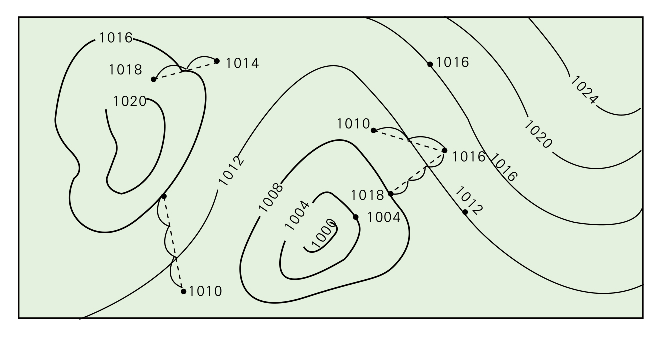
\includegraphics[width=0.8\linewidth]{Pictures/draw-weathermap01}
	\caption{등압선의 작도 방법}
	\label{fig:draw-weathermap01}
\end{figure}법

① 전선은 기온, 이슬점, 풍향이 불연속을 이루므로 이들 값이 급변하는 지역을 찾는다.
② 전선 상에서는 일반적으로 일기가 악화되므로 강수 등 나쁜 일기가 선상으로 나타날 경
우 전선이 존재할 가능성이 높다. 온난전선은 전면의 넓은 지역에서 강수 현상이 나타나
고 후면에는 비교적 맑은 날씨를 이룬다. 한랭전선은 전면과 후면의 구별 없이 전선 상에
서 비교적 좁은 지역에 강수 현상이 나타난다.
③ 전선이 확인되면 <그림 Ⅲ-22>와 같이 등압선이 휘도록 연결한다.

\begin{figure}
	\centering
	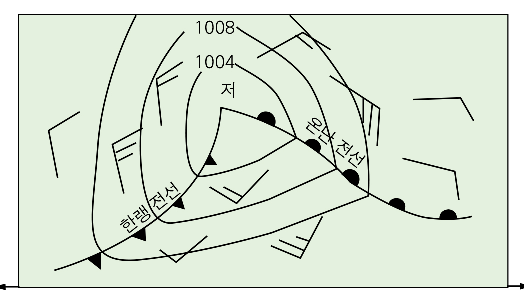
\includegraphics[width=0.8\linewidth]{Pictures/draw-weathermap02}
	\caption{전선에서의 등압선}
	\label{fig:draw-weathermap02}
\end{figure}



일기도 그리기
여러 가지 기상요소 중 간단한 등압선을 그리고 고·저기압의 위치 및 전선을 찾아 일기도를 완성해 보자.




\section{Corollaries}\index{Corollaries}

This is an example of a corollary.

\begin{corollary}[Corollary name]
	The concepts presented here are now in conventional employment in mathematics. Vector spaces are taken over the field $\mathbb{K}=\mathbb{R}$, however, established properties are easily extended to $\mathbb{K}=\mathbb{C}$.
	end{corollary}
	
	%------------------------------------------------
	
	\section{일기도 분석}\index{일기도 분석}
>>>>>>> feb34ee015c2e7337f28b19c6a5da86cd2e1c743
	
	기온, 강수 유무 등의 매일의 일기는 산업과 일상생활에 많은 영향을 미친다. 따라서 오랜
	세월 동안 일기를 정확히 예측하고자 많은 노력을 기울여 왔다. 아직도 많은 한계를 안고 있으
	나 날씨는 갑자기 변하는 것이 아니고 과거로부터 연속성을 가지고 변화하므로 과거와 현재의
	일기상태를 분석함으로써 미래의 일기를 어느 정도 예측할 수 있으며 보다 정확한 예측을 위
	하여 노력을 계속하고 있는 실정이다.
	일기의 분포는 일반적으로 기압배치에 대응되므로 기압배치를 예상할 수 있으면 일기예보
	가 어느 정도 가능하다. 고기압, 저기압의 기압계는 지속성을 가지고 있고, 우리나라 주변에서
	는 서에서 동으로 이동하므로 이를 이용하여 앞으로의 기압배치를 예측하고 날씨를 예상할 수
	있다. 고기압이 있는 지역의 지상일기는 하강 기류로 인해 구름이 소멸되어 맑은 날씨를 나타
	낸다. 반면 저기압지역에서는 내부의 상승기류로 인해 구름이 만들어지고 비가 내리게 되어
	궂은 날씨가 된다. 저기압은 전선을 동반하는 경우도 있는데 전선은 성질이 다른 두 기단의 경
	계를 이루는 상대적으로 좁은 영역을 이루므로 이 영역을 기준으로 온도나 바람 등이 급변할
	뿐 아니라 일반적으로 일기가 악화되어 강수 현상 등이 나타난다.
	
	\begin{figure}
		\centering
		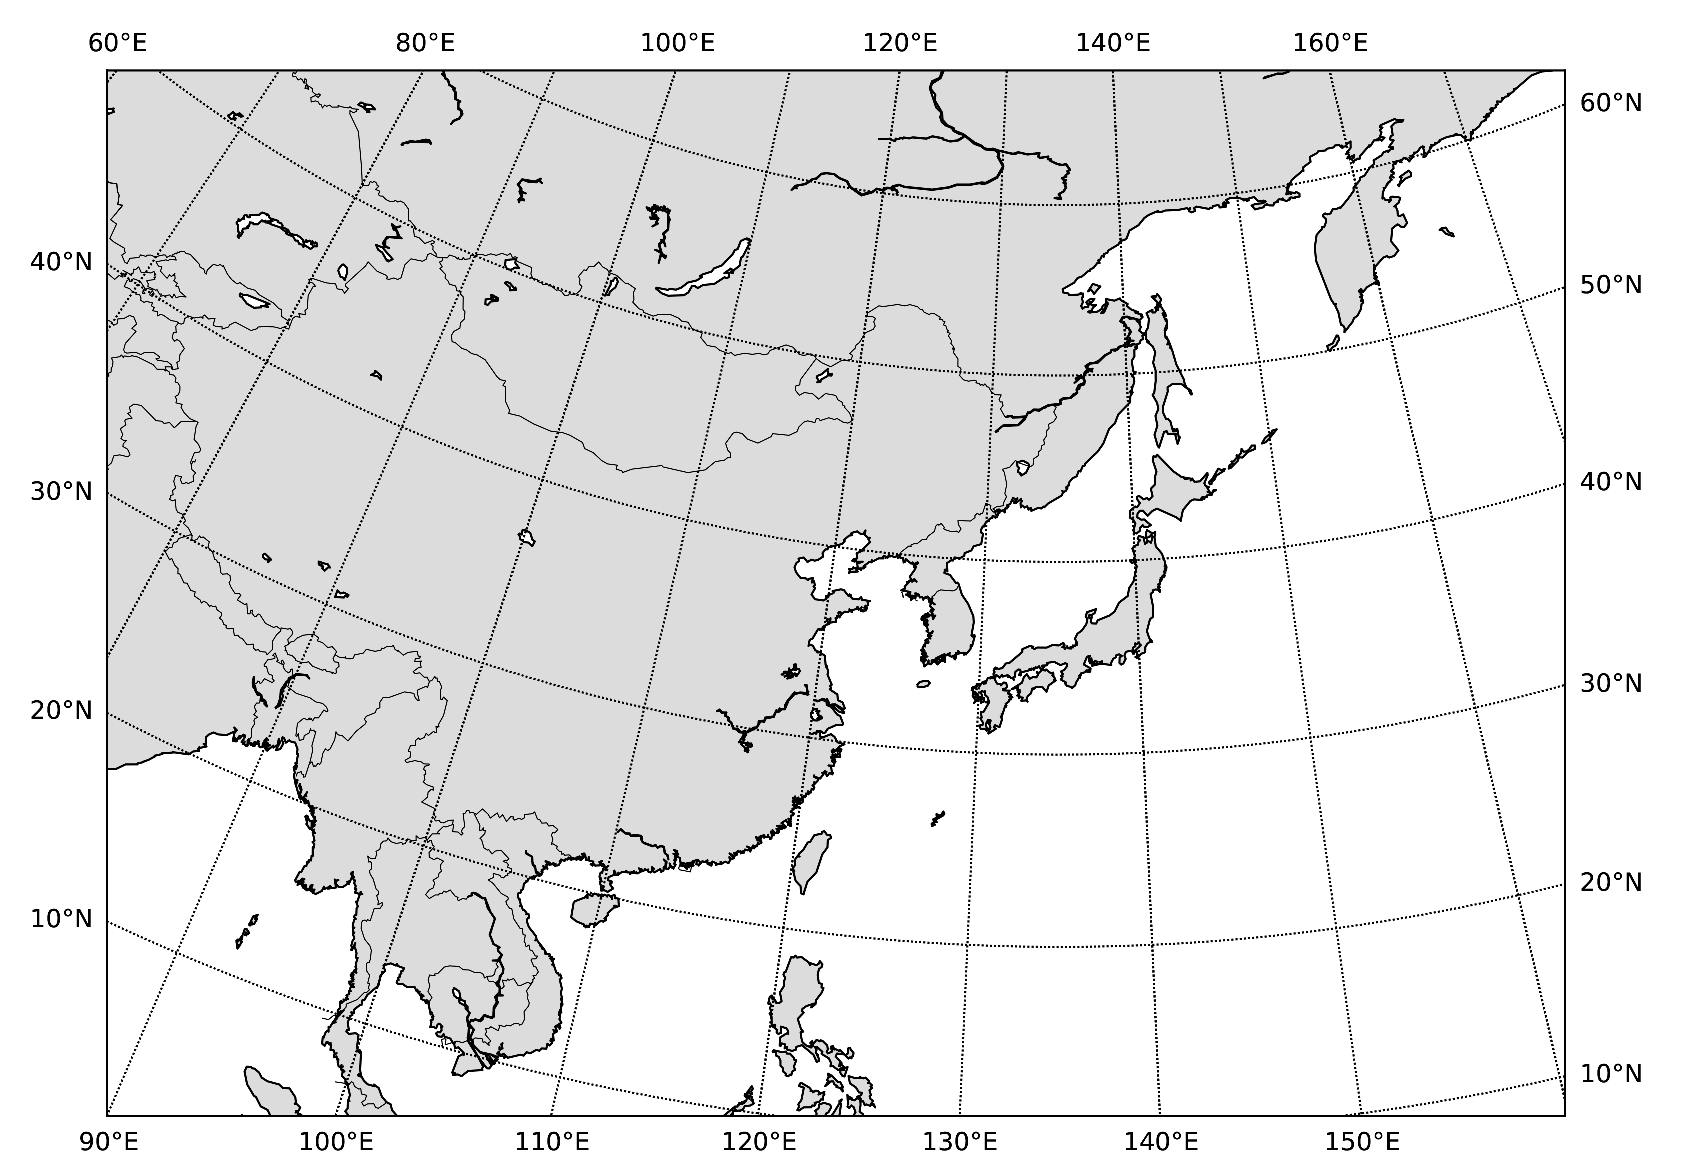
\includegraphics[width=0.8\linewidth]{Pictures/weathermap01}
		\caption{태풍이 이동하는 일기도}
		\label{fig:weathermap01}
	\end{figure}
	
	
	실제로 일기도가 완성되면 예보관은 이를 다각적으로 분석한다. 일기도의 분석은 고기압과
	저기압의 위치 및 이동경로, 기압과 고도의 변화경향, 전선의 발생 및 소멸과 이동 추적, 날씨
	변화, 대기의 연직구조 등을 세밀히 분석한다. 또한 특수기상 관측 자료인 기상레이더에 의한
	강수구역 추적, 기상위성에 의한 구름사진 분석, 자동기상관측자료(AWS) 등을 분석하여 앞으
	로의 날씨변화를 예상하게 된다. 또한 최근에는 컴퓨터를 활용하여 짧은 시간에 많은 기상자
	료를 처리할 수 있게 됨으로써 수치분석자료와 각종 보조일기도들을 이용할 수 있게 되어 정
	확한 날씨를 판단하는데 많은 도움을 주고 있다.
	
	\subsection{예상일기도 그리기}\index{Propositions!Several Equations}
	
	연속적인 몇 장의 일기도를 분석하여 앞으로 전개될 대기 상태를 예측하여 예상 일기도를 그려 보자.
	
	1. <그림 1>~<그림 4>는 2007년 7월 1일 6시부터 2일 18시까지 12시간 간격으로 연속 4회 동안 관
	측하여 작성한 지상일기도이다.
	⑴ 일기도 상에 나타난 전선을 다음 그림에 그려 넣고, 전선이 어느 방향으로 얼마나 이동했으며 평
	균 이동 속도는 얼마인지 다음 표를 작성하라. (단, 경도 1°의 거리는 위도 30°에서 96.5 km, 위도
	40°에서 85.4 km, 위도 50°에서 71.7 km이다. 위도 1°사이의 거리는 약 110 km이다.)
	
	
	⑵ 7월 3일 6시에는 기압계가 어떻게 달라졌을지 예상하여 다음 그림에 예상 일기도를 그려 보자.
	
	⑶ 다음 표는  기상청에서 발표한 7월 1일과 2일의 예보 통보문이다. 그린 예상 일기도를 바탕으로 예보 통보문을 작성해 보자.
	
	\begin{tabular}{|c|c|}
		\hline 
		일시	& 예보 통보문 \\ 
		\hline 
		7월 1일	& 동해상에 위치한 고기압 가장자리에 들겠습니다.
		전국이 대체로 구름 많고, 경상북도 지방은 새벽까지, 전라남북도 지방에서 아침까지 소
		나기(강수확률 60{\%})가 오는 곳이 있겠고, 오후에는 대기불안정으로 남부 내륙지방을 중
		심으로 산발적으로 소나기(강수확률 60{\%}가 오는 곳이 있겠습니다. \\ 
		\hline 
		7월 2일	& 서쪽에서 접근하는 장마전선의 영향을 점차 받겠습니다.
		전국이 대체로 흐리고 새벽에 중부서해안지방부터 비(강수확률 60~ 90{\%}가 시작되어 밤
		에는 전국으로 확대되겠습니다. \\ 
		\hline 
		7월 3일	&  \\ 
		\hline 
	\end{tabular} 





%----------------------------------------------------------------------------------------
%	CHAPTER 
%----------------------------------------------------------------------------------------

\chapterimage{chapter_head_1.pdf} % Chapter heading image

\chapter{기상청(www.kma.go.kr) 일기 예보}

\section{기상청 일기 예보의 종류}


\subsection{초단기 동네 예보}
초단기예보는 현재부터 앞으로 3시간까지, 실황(날씨, 기온, 습도 등 7개 요소)과 예보(강수형태, 하늘상태, 강수량 등 3개 요소)를 1시간 간격으로 동네예보를 기반으로 매 시각 30분에 발표한다. 초단기예보는 짧은 시간에 발생·소멸하는 기상현상에 대해 신속하게 대응하여 재해예방에 최선을 다하고자 2010년 6월 15일부터 홈페이지를 통해 제공하고 있다.

\subsection{동네 예보}
대상기간과 구역을 시ㆍ공간적으로 세분화하여 발표하는 예보로 기온, 최고기온, 최저기온, 강수형태, 강수확률, 12시간강수량, 12시간적설, 하늘상태, 습도, 풍향, 풍속, 파고 등을 예보한다. 동네예보는 3시간 간격으로 1일에 8회 예보하며 예보구간도 역시 3시간 단위로 48시간까지 예보한다. 

\subsection{주간 예보}
기상전망, 예보구역별 육상 및 해상 날씨, 지점별 기온, 파고에 대한 48시간 이후부터  6일간의 예보로 일 2회 발표(06시, 18시)하는 주간예보(모레부터 6일간)가 계속 유지될 가능성에 대한 신뢰도 정보를 3단계로 구분하여 제공(육상)한다.

\begin{table}[h]
	\centering
	\caption{신뢰도와 의미}
	\begin{tabular*}{.8\linewidth}{c|c}
		\hline 
		신뢰도  &	내용	  \\ 	\hline 
		높음  & 다음날 발표 주간예보가 계속 유지될 가능성이 높음  \\  \hline 
		보통 & 다음날 발표 주간예보가 계속 유지될 가능성이 있음  \\ 	\hline 
		낮음 & 다음날 발표 주간예보가 계속 유지될 가능성이 낮음   \\ 	\hline 
	\end{tabular*} 
\end{table}

\subsection{주말 예보}
토요일과 일요일의 기상 개황, 일별 날씨, 야외활동 지수 등의 정보를 제공한다. 화요일 19시부터 금요일 24시까지 제공되며, 매일 19시에 발표한다.

\subsection{장기 예보}
장기예보는 11일 이상에 대한 예보를 일컬으며 순별·월별 기압계 동향 및 전망, 기온·강수량 예보 등을 발표한다. 예보구역은 한반도 12개 권역(서울·인천·경기도, 강원도 영서, 강원도 영동, 대전·충청남도, 충청북도, 광주·전라남도, 전라북도, 부산·울산·경상남도, 대구·경상북도, 제주도, 평안남북도·황해도, 함경남북도)이며, 월 3회 발표되는 1월 전망과 월 1회 발표되는 3개월 전망이 있다. 그 외 연 4회 발표되는 기후전망은 다음다음 계절에 대한 전망으로 봄철 기후전망은 11월 23일 경에, 여름철 기후전망은 2월 23일 경에, 가을철 기후전망은 5월 23일 경에 겨울철 기후전망은 8월 23일 경에 발표한다.

